\documentclass[state=Thesis]{mcidoc}
% Preserve the % line endings in this configuration.
\newif\ifMCIBioscience
\MCIBiosciencefalse

\SetMCI{%
  StudentName = {Name = {OFFEN: Vorname Nachname}},%
  StudentID   = {OFFEN: Matrikelnummer},%
  Degree      = BSc,% BSc -> bachelor's; MSc -> master's thesis.
  Language    = DE,% German thesis: German + English abstracts.
  Department  = MECH,% Check applicability for another department.
  Title       = {OFFEN: Titel der Abschlussarbeit},%
  Thesis = {%
    StudyProgram = {OFFEN: Studiengang},%
    Supervisor = {%
      Name = {OFFEN: Betreuung}, Prefix = {}, Postfix = {},%
    },%
    Location = {Innsbruck},%
    Date     = {OFFEN: Datum},% Actual signing date; not the build date.
    Novelty  = set,% Class declaration, review before signing.
    Embargo  = unset,% Enable only an approved embargo.
    ToC = {Primary = set, Figures = set, Tables = set},%
    Bibliography = {Print = unset},% Printed explicitly in main.tex.
  },%
}

\usepackage{mci-template}
\addbibresource{references.bib}
\graphicspath{{figures/}}

% Required for a German-language thesis; print order is German, then English.
% These environments write auxiliary files; keep each end command on its own line.
\begin{Abstract}{DE}
\offen{Die Kurzfassung mit Problemstellung, Zielsetzung, Methode,
wichtigsten Ergebnissen und Schlussfolgerung verfassen.}
Der Text wird als eigenständige Zusammenfassung ohne Verweise auf
Abbildungen oder Kapitel formuliert. Die Vorlage enthält keine tatsächlichen
Forschungsergebnisse; die Beispiele im Hauptteil dienen nur dem Satz.
\end{Abstract}

\begin{Abstract}{EN}
\textit{OPEN: Replace this paragraph with the problem, objective, method,
principal results and conclusion of the completed thesis.}
The abstract must stand on its own and agree with the German summary.
The numerical examples in this template are synthetic and do not represent
experimental findings.
\end{Abstract}

% Optional: uncomment the COMPLETE environment if desired.
% \begin{Acknowledgments}
% OFFEN: Persönliche Danksagung einfügen oder diesen Block entfernen.
% \end{Acknowledgments}
%

\begin{document}
\chapter{Einleitung}
\label{chap:introduction}

\section{Problemstellung und Motivation}
\offen{Das fachliche Problem, den Anwendungskontext und die Relevanz
anhand belastbarer Quellen beschreiben.}
Der Gegenstand der Arbeit wird eingegrenzt. Offene technische Fragen
werden von bereits bekannten Zusammenhängen unterschieden.

\section{Zielsetzung und Forschungsfrage}
\offen{Eine präzise Forschungsfrage und überprüfbare Ziele formulieren.
Nicht untersuchte Aspekte und Randbedingungen benennen.}
Es wird beschrieben, anhand welcher Kriterien die Ergebnisse später
bewertet werden.

\section{Aufbau der Arbeit}
Die Grundlagen werden in Kapitel~\ref{chap:background} behandelt.
In Kapitel~\ref{chap:methods} wird die Methodik dargestellt.
Die Ergebnisse in Kapitel~\ref{chap:results} werden in
Kapitel~\ref{chap:discussion} diskutiert. Die Arbeit wird mit
Kapitel~\ref{chap:conclusion} abgeschlossen. Ergänzende Unterlagen werden
in Anhang~\ref{app:records} gesammelt.

\chapter{Grundlagen und Stand der Technik}
\label{chap:background}

\section{Stand der Forschung}
\offen{Relevante Originalpublikationen vergleichen und die daraus
abgeleitete Forschungslücke belegen.}
Hier wird nur ein Zitierbeispiel gesetzt; der nachfolgende Beleg ist ein
ausdrücklich zu ersetzender Quellenplatzhalter.\mcicite{quelle-ersetzen}
Quellen werden möglichst unmittelbar nach der übernommenen Aussage
angegeben und im Verzeichnis nach ihrer Erstnennung geordnet.

\section{Modell und Formelzeichen}
Die folgenden Kapitel enthalten ein eigenständig gekennzeichnetes
Vorlagenbeispiel mit synthetischen Daten. Es werden keine durchgeführten
Messungen behauptet. Als Satzbeispiel wird in \eqnref{eq:ohm} ein ohmsches
Modell bei konstanter Temperatur verwendet:
\begin{equation}
  R = \frac{U}{I}.
  \label{eq:ohm}
\end{equation}
Dabei steht $R$ für den elektrischen Widerstand in \unit{\ohm}, $U$ für
die Spannung in \unit{\volt} und $I$ für die Stromstärke in \unit{\ampere}.
\offen{Das für die Forschungsfrage geeignete Modell fachlich belegen,
seine Annahmen prüfen und alle verwendeten Zeichen erläutern.}

Kurze Direktzitate können mit \mciquote{OFFEN: exakter Originalwortlaut}
gesetzt werden. Quelle und genaue Fundstelle werden ergänzt; auch
Paraphrasen und übernommene Gliederungen erhalten einen Beleg.

\chapter{Materialien und Methoden}
\label{chap:methods}

\begin{mcimethods}
\section{Materialien und Geräte}
\offen{Gerätemodelle, Messbereiche, Auflösung, Kalibrierstatus und
Unsicherheiten dokumentieren. Für Chemikalien außerdem Bezeichnung,
Konzentration, Reinheit und eingesetzte Mengen ergänzen.}
Alle für die Reproduktion wesentlichen Angaben werden aus der tatsächlichen
Versuchsdokumentation übernommen.

\section{Versuchsaufbau}
In \figref{fig:setup} wird ein schematischer Beispielaufbau gezeigt.
Die Skizze wird vor der Abgabe durch den tatsächlichen, beschrifteten
Aufbau ersetzt.
\begin{figure}[htbp]
  \centering
  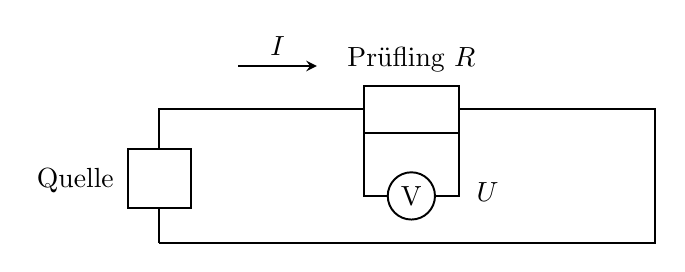
\begin{tikzpicture}[line width=0.7pt,>=stealth]
    \draw (0,0) -- (0,1.7) -- (2.6,1.7);
    \draw (3.8,1.7) -- (6.3,1.7) -- (6.3,0) -- (0,0);
    \draw[fill=white] (-0.4,0.45) rectangle (0.4,1.2);
    \node[left] at (-0.45,0.8) {Quelle};
    \draw[fill=white] (2.6,1.4) rectangle (3.8,2.0);
    \node[above] at (3.2,2.05) {Prüfling $R$};
    \draw[->] (1,2.25) -- (2,2.25) node[midway,above] {$I$};
    \draw (2.6,1.7) -- (2.6,0.6) -- (2.9,0.6);
    \draw (3.5,0.6) -- (3.8,0.6) -- (3.8,1.7);
    \draw[fill=white] (3.2,0.6) circle (0.3);
    \node at (3.2,0.6) {V};
    \node[right] at (3.9,0.65) {$U$};
  \end{tikzpicture}
  \caption[Beispiel einer Versuchsskizze]{Schematischer Beispielaufbau mit
    Quelle, Prüfling und Spannungsmessung. Eigene Darstellung; reale
    Gerätedetails und Strommessung ergänzen.}
  \label{fig:setup}
\end{figure}

\section{Durchführung und Auswertung}
\offen{Arbeitsschritte, Umgebungsbedingungen, Wiederholungen und
Auswertungsverfahren reproduzierbar beschreiben.}
Direkt erfasste Größen und berechnete Werte werden unterschieden.
Für jeden unterschiedlichen Rechenschritt wird ein Zahlenbeispiel gezeigt.
Ergänzende Unterlagen sind in Anhang~\ref{app:records} aufgeführt.
\end{mcimethods}

\chapter{Ergebnisse}
\label{chap:results}

\section{Darstellung der Daten}
In \tabref{tab:example} werden synthetische Beispieldaten zur Demonstration
von Einheiten, Dezimalstellen und Unsicherheiten gezeigt. Die Unsicherheiten
sind hier als Standardunsicherheiten definiert; ihre Werte sind für dieses
Satzbeispiel frei gewählt.
\begin{table}[htbp]
  \centering
  \caption[Synthetische Beispieldaten]{Synthetische Beispieldaten, keine
    Messwerte. $u_U$ und $u_I$ bezeichnen die zugeordneten
    Standardunsicherheiten von Spannung und Stromstärke.}
  \label{tab:example}
  \begin{tabular}{c S[table-format=1.3] S[table-format=1.3]
                    S[table-format=2.2] S[table-format=1.2]}
    \toprule
    Nr. & {$U/\unit{\volt}$} & {$u_U/\unit{\volt}$}
        & {$I/\unit{\milli\ampere}$} & {$u_I/\unit{\milli\ampere}$} \\
    \midrule
    1 & 1.000 & 0.005 & 10.00 & 0.10 \\
    2 & 2.000 & 0.005 & 20.00 & 0.10 \\
    3 & 3.000 & 0.005 & 30.00 & 0.10 \\
    \bottomrule
  \end{tabular}
\end{table}

In \figref{fig:example-plot} werden dieselben Punkte mit horizontalen und
vertikalen Fehlerbalken dargestellt. Die gestrichelte Modellgerade wird
mit dem vorgegebenen Beispielwert $R=\qty{100}{\ohm}$ gezeichnet; sie ist
keine Regression. Die kleinen Fehlerbalken entsprechen den Beispielwerten
und werden nicht künstlich vergrößert.
\begin{figure}[htbp]
  \centering
  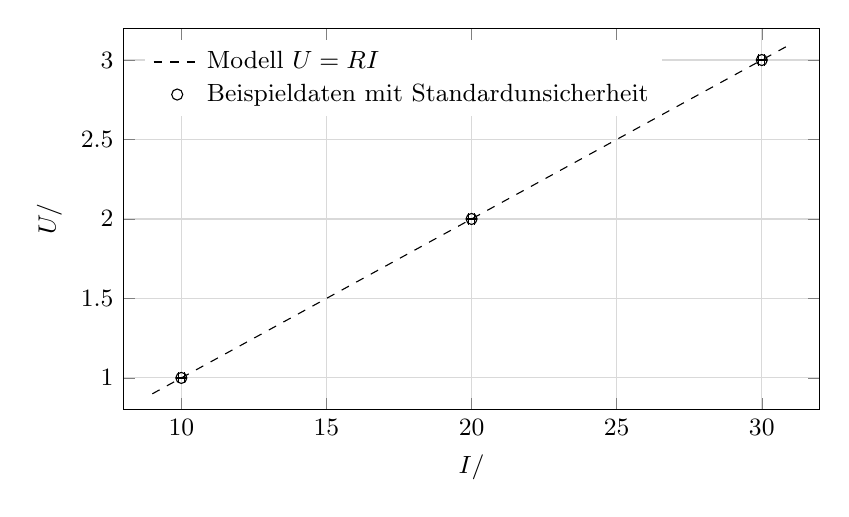
\begin{tikzpicture}
    \begin{axis}[
      width=0.86\linewidth,height=0.53\linewidth,
      xlabel={$I/\unit{\milli\ampere}$},ylabel={$U/\unit{\volt}$},
      xmin=8,xmax=32,ymin=0.8,ymax=3.2,
      xtick={10,15,20,25,30},ytick={1,1.5,2,2.5,3},
      grid=major,grid style={black!15},
      legend pos=north west,legend cell align=left,
      tick label style={font=\small},label style={font=\small},
      legend style={font=\small,draw=none},
    ]
      \addplot[black,dashed,domain=9:31,samples=2] {0.1*x};
      \addlegendentry{Modell $U=RI$}
      \addplot[only marks,mark=o,black,
        error bars/.cd,x dir=both,x explicit,y dir=both,y explicit]
        coordinates {(10,1) +- (0.1,0.005)
                     (20,2) +- (0.1,0.005)
                     (30,3) +- (0.1,0.005)};
      \addlegendentry{Beispieldaten mit Standardunsicherheit}
    \end{axis}
  \end{tikzpicture}
  \caption[Beispieldaten mit Modellgerade]{Synthetische Beispieldaten
    (Kreise mit Fehlerbalken) und vorgegebene Modellgerade (gestrichelt).
    Eigene Darstellung; keine experimentellen Ergebnisse.}
  \label{fig:example-plot}
\end{figure}

\section{Vollständige Beispielrechnung}
Für Zeile 1 in \tabref{tab:example} wird mit \eqnref{eq:ohm} gerechnet:
\begin{equation}
  R = \frac{U}{I}
    = \frac{\qty{1.000}{\volt}}{\qty{10.00e-3}{\ampere}}
    = \qty{100.0}{\ohm}.
  \label{eq:calculation}
\end{equation}
\eqnref{eq:calculation} zeigt Ansatz, eingesetzte Werte und Ergebnis.
Nur für unkorrelierte Eingangsgrößen und bei zulässiger linearer
Unsicherheitsfortpflanzung ergibt sich hier nach \eqnref{eq:uncertainty}
die kombinierte Standardunsicherheit $u_R$ in \unit{\ohm}:
\begin{equation}
  \begin{aligned}
    u_R &= R\sqrt{\left(\frac{u_U}{U}\right)^2
                    +\left(\frac{u_I}{I}\right)^2} \\
        &= \qty{100.0}{\ohm}
           \sqrt{\left(\frac{\qty{0.005}{\volt}}{\qty{1.000}{\volt}}\right)^2
                +\left(\frac{\qty{0.10}{\milli\ampere}}{\qty{10.00}{\milli\ampere}}\right)^2}
         \approx \qty{1.1}{\ohm}.
  \end{aligned}
  \label{eq:uncertainty}
\end{equation}
Damit wird das Beispielergebnis als
$R=\qty{100.0 +- 1.1}{\ohm}$ angegeben. Die Schreibweise bezeichnet hier
die Standardunsicherheit, kein erweitertes Vertrauensintervall.
\offen{Die verwendete Unsicherheitsmethode fachlich belegen und die
Annahmen anhand der realen Messung prüfen.}

\section{Ergebnisübersicht}
\offen{Die tatsächlichen Ergebnisse zur Forschungsfrage darstellen.
Ihre fachliche Bewertung und die Grenzen werden im folgenden
Diskussionskapitel behandelt.}

\chapter{Diskussion}
\label{chap:discussion}

\section{Beantwortung der Forschungsfrage}
\offen{Die tatsächlichen Ergebnisse anhand der in der Einleitung
festgelegten Kriterien bewerten und die Forschungsfrage beantworten.}
Beobachtungen werden von ihrer Interpretation unterschieden.
Synthetische Vorlagendaten werden nicht als Evidenz herangezogen.

\section{Einordnung und Grenzen}
\offen{Ergebnisse mit Originalpublikationen vergleichen, systematische
Effekte und Unsicherheiten diskutieren und die Übertragbarkeit eingrenzen.}
Es wird erläutert, welche Aussagen durch die Daten gestützt werden und
welche weiteren Untersuchungen für offene Fragen erforderlich sind.

\chapter{Fazit und Ausblick}
\label{chap:conclusion}

\offen{Die wichtigsten nachgewiesenen Erkenntnisse, den Beitrag der Arbeit
und die Zielerreichung präzise zusammenfassen.}
Die Schlussfolgerung wird aus den zuvor dargestellten Ergebnissen und
ihrer Diskussion abgeleitet. Neue Daten oder unbelegte Aussagen werden
nicht eingeführt.

\offen{Konkrete nächste Forschungsschritte aus den verbleibenden Grenzen
ableiten.}


\printbibliography[heading=bibintoc,title={\MCIText{Quellenverzeichnis}{References}}]
\MCIPrintBackMatter
\addchap{\MCIText{Formelzeichenübersicht}{List of symbols}}
% One row per base symbol; do not repeat u_U, u_I, u_R as separate variants.
\begin{longtable}{@{}p{0.12\textwidth}p{0.57\textwidth}p{0.23\textwidth}@{}}
  \toprule
  \MCIText{Zeichen}{Symbol} & \MCIText{Bedeutung}{Description}
    & \MCIText{Einheit}{Unit} \\
  \midrule
  \endhead
  $I$ & Elektrische Stromstärke & \unit{\ampere} \\
  $R$ & Elektrischer Widerstand & \unit{\ohm} \\
  $U$ & Elektrische Spannung & \unit{\volt} \\
  $u$ & Standardunsicherheit einer Größe; Einheit wie Bezugsgröße
      & \unit{\ampere}, \unit{\ohm} oder \unit{\volt} \\
  \bottomrule
\end{longtable}
\noindent Es werden keine physikalischen Konstanten im Vorlagenbeispiel
verwendet. \offen{Bei Bedarf verwendete physikalische Konstanten mit
Wert, Einheit und Quelle ergänzen.}

\appendix
\chapter{Ergänzende Unterlagen}
\label{app:records}

\offen{Rohdaten, Versuchsprotokoll, ergänzende Rechnungen oder relevante
Auszüge der Aufgabenstellung ergänzen.}
Der Anhang wird im Haupttext an der passenden Stelle referenziert,
beispielsweise als Anhang~\ref{app:records}. Externe Unterlagen erhalten
einen Quellenverweis. Die römische Seitenzählung wird aus dem vorderen
Dokumentteil fortgesetzt.

\end{document}
